% ОБЯЗАТЕЛЬНО ИМЕННО ТАКОЙ documentclass!
% (Основной кегль = 14pt, поэтому необходим extsizes)
% Формат, разумеется, А4
% article потому что стандарт не подразумевает разделов
% Глава = section, Параграф = subsection
% (понятия "глава" и "параграф" из стандарта)
\documentclass[a4paper,article,14pt]{extarticle}

% Подключаем главный пакет со всем необходимым
\usepackage{spbudiploma_tempora}

% Пакеты по желанию (самые распространенные)
% Хитрые мат. символы
\usepackage{euscript}
% Таблицы
\usepackage{longtable}
\usepackage{makecell}
% Картинки (можно встявлять даже pdf)
\usepackage[pdftex]{graphicx}

\usepackage{amsthm,amssymb, amsmath}
\usepackage{textcomp}
\usepackage{dsfont}

\begin{document}

% Титульник в файле titlepage.tex
% Титульный лист диплома СПбГУ
% Временное удаление foot на titlepage
\newgeometry{left=30mm, top=20mm, right=15mm, bottom=20mm, nohead, nofoot}
\begin{titlepage}
\begin{center}
% Первый символ съедается, первым знаком поставлен Ы
\textbf{Санкт--Петербургский}
\textbf{государственный университет}

\vspace{35mm}

\textbf{\textit{\large Тихонков Сергей Алексеевич}} \\[8mm]
% Название
\textbf{\large Выпускная квалификационная работа}\\[3mm]
\textbf{\textit{\large Исследование и применение алгоритмов на базе консенсуса для распределенного обучения нейронных сетей}}

\vspace{20mm}
% Булшит
Уровень образования: бакалавриат\\
Направление 02.03.02 «Фундаментальная информатика и информационные технологии»\\
Основная образовательная программа СВ.5003.2017
«Программирование и информационные технологии»\\
Профиль «Автоматизация научных исследований»\\[30mm]


% Научный руководитель, рецензент
% Сходить в уч отдел и узнать, правильно ли
\begin{flushright}
{Научный руководитель:} \\
профессор, кафедра математического моделирования энергетических систем, д.ф. - м.н.  Крылатов~Александр Юрьевич
\end{flushright}
\begin{flushright}
{Рецензент:} \\
доцент, зав. каф. компьютерных технологий и систем, к.ф. - м.н.  Погожев~Сергей Владимирович
\end{flushright}

\vfill 

{Санкт-Петербург}
\par{\the\year{} г.}
\end{center}
\end{titlepage}
% Возвращаем настройки geometry обратно (то, что объявлено в преамбуле)
\restoregeometry
% Добавляем 1 к счетчику страниц ПОСЛЕ titlepage, чтобы исключить 
% влияние titlepage environment
\addtocounter{page}{1}


% Содержание
\tableofcontents
\pagebreak

\specialsection{Введение}
С каждым годом растет количество
накопленных человечеством данных. Современное аппаратное обеспечение часто не позволяет проводить вычисления
с большим количеством данных на одной машине. Это часто связано во-первых, с ограниченным объемом оперативной памяти компьютера,
а во-вторых, с ограниченным временным на решение конкретной задачи. Область машинного обучения испытывает обе перечисленные проблемы.
Часто для достижения требуемого результата необходимо обучение нейронной сети с множеством параметров на огромном объеме данных.
Это препятствует прогрессу в исследованиях и разработках.  В связи с этим существует потребность в методах распределенного обучения.
Они позволяют не ограничиваться мощностями одной машины при конструировании новых методов в машинном обучении
и ускоряют уже существующие решения.

Помимо этого на практике часто возникает потребность обрабатывать информацию разной степени приватности. В некоторых случаях
при обучении нейронной сети используются данные, распространение которых запрещено или нежелательно. Отличным примером этого
является какой-либо совместный проект двух банков, в ходе которого они хотят решить общую задачу, но не могут передать, пусть даже
и обезличенные, данные своих клиентов друг другу. В этом случае возникает необходимость использовать методы распределенного обучения, которые
обеспечивают изоляцию данных.

Топология сети и методы взаимодействия узлов являются важными свойствами распределенных систем. Не всегда вычислительные
кластеры имеют регулярную структуру, часто доступные вычислительные ресурсы представляют собой гетерогенную компьютерную сеть,
где пропускная способность каналов связи и мощности каждого узла могут сильно отличаться. В этом случае применяемые методы распределенного
обучения должны быть устойчивы к неоднородности сети.

В данной работе проводится краткий обзор основных методов распределенного обучения нейронных сетей и исследование
возможности применения алгоритма на базе консенсуса для распределенного обучения с изоляцией данных. Также рассматривается
способность исследуемого алгоритма корректно решать задачу в сети с неоднородной вычислительной мощностью узлов.
\pagebreak

\specialsection{Постановка задачи}
Целью данной работы является исследование возможности применения алгоритма на базе консенсуса для распределенного
обучения нейронных сетей. Для достижения поставленной цели были сформулированны следующие задачи:

\begin{itemize}
  \item изучение предметной области и обзор существующих методов
  \item изучение математической теории, описывающей исследуемый подход
  \item реализация алгоритма и прототипа распределенной сети для проведения экспериментов
  \item проведение экспериментов и анализ результатов
\end{itemize}
\pagebreak

\section{Обзор}
\subsection{Обзор раз}
Ненумерованная формула:

\begin{equation}
    \begin{pmatrix} \dot{\varphi}\\ \dot{\theta} \\ \dot{\psi} \end{pmatrix}
    = \begin{pmatrix}
        cos(\theta)cos(\psi) & -sin(\psi) & 0 \\
        cos(\theta)sin(\psi) & cos(\psi)  & 0 \\
        -sin(\theta)         & 0         &  1
    \end{pmatrix}^{-1}
    \begin{pmatrix} \omega_x\\ \omega_y \\ \omega_z \end{pmatrix}.
\end{equation}

Нумерованная формула:

\begin{equation} \label{eq:my_ref}
    i^2 = -1.
\end{equation}

Тест ссылки на формулу~\ref{eq:my_ref}!

\subsection{Обзор два}

\subsection{Обзор три}
Ниже тестируется очень большая таблица на несколько страниц

\begin{center}
    \begin{longtable}{|p{2cm}|p{3cm}|p{7cm}|p{3cm}|}
    \caption{Заголовок таблицы}\\
    \hline
    1 & 2 & 3 & 4\\
    \hline
    2 & 2 & 3 & 4\\
    \hline
    3 & 2 & 3 & 4\\
    \hline
    4 & 2 & 3 & 4\\
    \hline
    5 & 2 & 3 & 4\\
    \hline
    6 & 2 & 3 & 4\\
    \hline
    7 & 2 & 3 & 4\\
    \hline
    8 & 2 & 3 & 4\\
    \hline
    9 & 2 & 3 & 4\\
    \hline
    10 & 2 & 3 & 4\\
    \hline


    \end{longtable}
\end{center}


А также тестируется счетчик таблиц, жирные и двойные линии.

\begin{center}
    \begin{longtable}{|p{2cm}||p{3cm}|p{7cm}|p{3cm}|}
    \caption{Заголовок таблицы нумер 2}\\
    \hline
    1 & 2 & 3 & 4\\
    \hline
    2 & 2 & 3 & 4\\
    \hline
    3 & 2 & очень жирная ячейка \par с переносом (работаеттт!) & 4\\
    \hline
    4 & 2 & 3 & 4\\
    \hline
    5 & 2 & 3 & 4\\
    \hline
    6 & 2 & 3 & 4\\
    \hline
    7 & 2 & 3 & 4\\
    \hline
    8 & 2 & 3 & 4\\
    \hline
    9 & 2 & 3 & 4\\
    \hline
    10 & 2 & 3 & 4\\
    \hline


    \end{longtable}
\end{center}

\section{Теория}
\subsection{Задача машинного обучения}
Вспомним стандартную постановку задачи машинного обучения: есть некоторое параметрическое семейство функций  $f(\bullet, \theta)$ и набор данных $(x_i, y_i)_{i=0}^{m-1}$, требуется подобрать параметры $\theta$ так, чтобы $f(\bullet, \theta)$ как можно лучше соответствовала этим данным.

Формулировка в виде задачи оптимизации:
 \begin{equation} \label{eq:ml_task}
 \mathcal{J}(\theta)=
 \frac{1}{m}\sum_{i=0}^{m-1}g(f(x_i, \theta), y_i)\rightarrow_{\theta}\min
 \end{equation}
где $g(f(x_i, \theta), y_i)$ -- функция ошибки.

Часто эту задачу решают с помощью пакетного градиентного спуска (Mini Batch Gradient Descent) \cite{mbgd}:
  \begin{equation} \label{eq:mbgd}
\theta_{k+1} = \theta_k - \alpha_k\frac{1}{|S_k|}\sum_{i\in S_k}\nabla g(f(x_i, \theta_k), y_i)
 \end{equation}
где $S_k$ –- случайно выбранное подмножество $\{0, \ldots, m-1\}$, $\alpha_k$ –- коэффициент скорости обучения.

\subsection{Алгоритм среднего консенсуса}

Алгоритм консенсуса -- это процесс в теории управления, используемый для достижения согласия по единому значению данных среди распределенных процессов или систем. То есть форма стабильной системы, в которой состояния $\pi(t)_i$ распределенной системы сошлись к одному значению:
\begin{equation}
\pi_i(t)\rightarrow \pi^*,~0\leq i\leq m-1.
\end{equation}

Базовый (средний) консенсус можно использовать для децентрализованного вычисления среднего нескольких чисел, каждое из которых хранится на отдельном вычислительном узле \cite{consensus_basics}:
\begin{equation}
x^0 = (x_1^0, \ldots, x_p^0)
\end{equation}
\begin{equation}
x_i^* = \frac{1}{p}\sum_{j=1}^{p}x_j^0.
\end{equation}

Рассмотрим сеть агентов, принимающих решения, с динамикой $\dot x_i = u_i$, заинтересованных в достижении консенсуса посредством локальной коммуникации со своими соседями на графе $G = (V, E)$.
То есть сходимости:
\begin{equation}
x_1 = x_2 = \ldots = x_n.
\end{equation}

Это может быть выражено как $x = \alpha \mathds{1} $, где $\mathds{1} = (1, \ldots, 1)^T$ и $\alpha \in R$ -- коллективное решение группы агентов. Пусть $A = a_{ij}$ -- матрица смежности графа $G$. Множество соседей агента $i$ -- это $N_i$ и определяется формулой
\begin{equation}
N_i = \{ j \in V: a_{ij} \ne 0 \}; \quad \quad V = \{1, \ldots, n\}.
\end{equation}

Агент $i$ коммуницирует с агентом $j$, если $j$ является соседом $i$. Набор всех узлов и их соседей определяет набор ребер графа
\begin{equation}
E = \{ (i,j) \in V\times V: a_{ij} \ne 0\}.
\end{equation}

Динамический граф $G(t) = (V, E(t))$ -- это граф, в котором набор ребер $E(t)$ и матрица смежности $A(t)$ изменяются во времени. Ясно, что множество соседей $N_i(t)$ каждого агента в динамическом графе также является изменяющимся во времени множеством.

В \cite{consensus_basics_2} показано, что линейная система
\begin{equation} \label{eq:system_dynamic}
\dot x_i(t) = \sum_{j \in N_i} a_{ij}(x_j(t)-x_i(t))
\end{equation}
представляет собой алгоритм распределенного консенсуса, т.е. гарантирует сходимость к коллективному решению через локальные межагентные взаимодействия. Предполагая, что граф неориентированный ($a_{ij}=a_{ji}, \forall i,j \in V$), следует, что сумма состояний всех узлов является инвариантной величиной, или $\sum_i \dot x_i = 0$. В частности, применив это условие для $t = 0 \text{ и } t = \infty$ получаем:
\begin{equation}
\alpha = \frac{1}{n}\sum_i x_i.
\end{equation}

Другими словами, если консенсус достигается асимптотически, то коллективное решение обязательно равно среднему значению начального состояния всех узлов.

В компактном виде изменения системы \ref{eq:system_dynamic} можно записать как
\begin{equation}
\dot x = -Lx
\end{equation}
где $L$ -- лапласиан графа $G$. По определению, $L$ имеет правый собственный вектор, равный $\mathds{1}$, связанный с нулевым собственным значением из-за тождества $L\mathds{1} = 0$. В случае неориентированных графов лапласиан графа удовлетворяет следующему свойству суммы квадратов (ССК):
\begin{equation} \label{eq:sos}
x^TLx = \frac{1}{2}\sum_{(i, j) \in E} a_{ij}(x_j-x_i)^2.
\end{equation}

Определив квадратичную функцию несогласия как
\begin{equation}
\varphi(x) = \frac{1}{2}x^TLx
\end{equation}
становится ясно, что алгоритм \ref{eq:system_dynamic} такой же, как
\begin{equation}
\dot x = -\nabla \varphi(x)
\end{equation}
или алгоритм градиентного спуска. Этот алгоритм асимптотически сходится при соблюдении двух условий: 1) $L$ - положительно полуопределенная матрица; 2) единственное решение системы \ref{eq:system_dynamic} это $\alpha \mathds{1}$ для некоторого $\alpha$. Оба эти условия выполняются для связного графа и следуют из ССК-свойства лапласиана графа в \ref{eq:sos}. Следовательно, средний консенсус достигается асимптотически для всех начальных состояний. Этот факт резюмируется в \cite{consensus_basics} следующей леммой:

\textit{Лемма 1}: Пусть $G$ - связный неориентированный граф. Тогда алгоритм \ref{eq:system_dynamic} асимптотически решает задачу среднего консенсуса для всех начальных состояний.

\subsection{Быстрая сходимость}
Выяснив, что алгоритм \ref{eq:system_dynamic} асимптотически решает задачу среднего консенсуса, можно задаться вопросом о скорости его сходимости. В \cite{fast_averaging} говорится о том, что можно выбрать такие веса $a_{ij}$ ребер графа $G$, чтобы алгоритм сходился с максимальной скоростью. Для этого необходимо решить задачу оптимизации, в которой максимизируется второе из минимальных собственных значений лапласиана $L$ графа $G$ при известных ограничениях на веса ребер. Стоит отметить, что второе собственное значение лапласиана графа возникает из теории графов и называется алгебраическая связность.


\subsection{Консенсус и задача МО}
Применим алгоритм среднего консенсуса к задаче машинного обучения. Пусть каждый вычислительный узел идентифицирован своим индексом $t = \{1, \ldots, p \}$ и хранит свою копию параметров $\theta^t$. Происходит разделение исходных данных $S = \cup_{t=1}^p S^t$, причем $S_i \cup S^j = \oslash \text{ для } i \ne j$. Каждое $S^t$ является множеством исходных данных соответствующего узла $t$. Тогда, в соответствии с \cite{decentralized_sgd}, каждый шаг алгоритма для каждого агента $t$ будет выглядеть как:
\begin{itemize}
\item
    Обучить текущие веса $\theta_k^t$ на подмножестве локальных данных:
     \begin{equation} \label{eq:algo_step_1}
    \theta_{k+\frac{1}{2}}^t =
    \theta_k^t - \alpha_k\frac{1}{|S_k^t|}\sum_{i\in S_k^t}\nabla g(f(x_i, \theta_k), y_i)
    \end{equation}

\item
    Сделать консенсусное усреднение параметров с соседями:
     \begin{equation} \label{eq:algo_step_2}
     \theta_{k+1}^t =
     \sum_{i \in N_t}a_{pi}\theta_{k+\frac{1}{2}}^i
     \end{equation}
где $N_t$ -- соседи узла $t$, причем $t \in N_t$.
\end{itemize}

Шаг \ref{eq:algo_step_1} отличается от стандартного подхода \ref{eq:mbgd} только тем, что множество $S_k^t$ зависит от $t$, эти множества не пересекаются для разных $t$, то есть происходит разделение данных между вычислительными узлами.

Шаг \ref{eq:algo_step_2} –- усреднение параметров модели  между соседними узлами. Здесь происходит обмен информацией между узлами, причем этот шаг не обязан выполняться каждую итерацию.

Как следует из теории, изложенной в предыдущем параграфе, эти шаги эквивалентны обучению одиночной модели с использованием батча $S_k^1 \cup S_k^2 \cup \ldots \cup S_k^p$.

В случае распределенного обучения нейронных сетей под достижением консенсуса мы подразумеваем асимптотическую сходимость параметров моделей на каждом узле $\theta_1^*=\theta_2^*=\ldots=\theta_p^*$.
Однако на практике удобно не отслеживать факт достижения консенсуса с какой-то точностью, а делать конечное количество итераций, заданное вначале.


\pagebreak
\section{Алгоритм}
\subsection{Средний консенсус}
\subsection{Консенсус с несбалансированными данными}

\section{Эксперименты}
\subsection{Выбор модели и датасета}
\subsection{Преобразование данных}
\subsection{LSR}
\subsection{warmup}
\subsection{Топология сети}
Про экспандеры, разное количество диагоналей в цикле и вцелом про то какие топологии хорошие

\subsection{Анализ экспериментов}
\begin{figure}[ht]
\begin{center}
\scalebox{0.4}{
   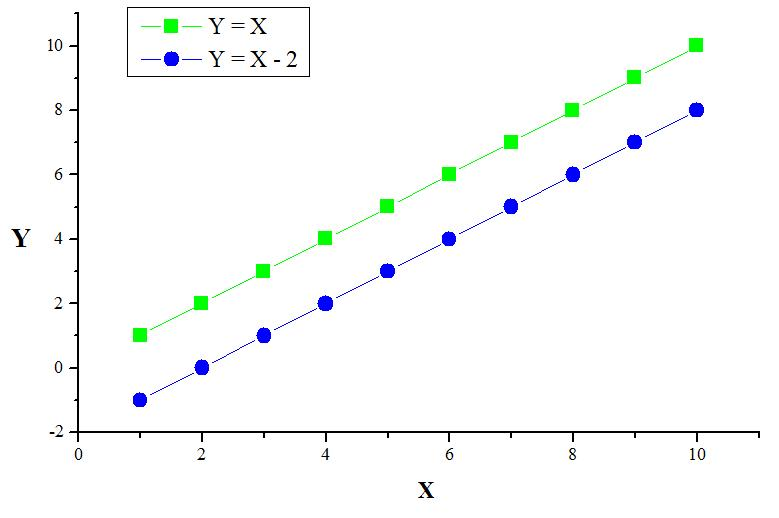
\includegraphics{examples/images/graph.jpg}
}

\caption{
\label{graph-fig}
     Линейные функции.}
\end {center}
\end {figure}
Ссылаемся на график ~\ref{graph-fig}.
Ссылка на статью: \cite{mbgd}

\specialsection{Выводы}
Жизнь --- тлен.
\pagebreak

\specialsection{Заключение}

% Библиография в cpsconf стиле
% Аргумент {1} ниже включает переопределенный стиль с выравниванием слева
\begin{thebibliography}{1}
\bibitem{mbgd} S. Ghadimi, G. Lan, and H. Zhang. \flqq Mini-batch stochastic approximation methods for nonconvex stochastic composite optimization\frqq. Mathematical Programming, 2016. // URL: https://link.springer.com/content/pdf/10.1007/s10107-014-0846-1.pdf

\bibitem{consensus_basics} R Olfati-Saber, JA Fax, RM Murray. \flqq Consensus and cooperation in networked multi-agent systems \frqq. IEEE, 2007.

\bibitem{consensus_basics_2} R. Olfati-Saber and R. M. Murray, \flqq Consensus problems in networks of agents with switching topology and time-delays \frqq. IEEE Transactions on Automatic Control, vol. 49, no. 9, pp. 1520-1533, Sept. 2004, doi: 10.1109/TAC.2004.834113.

\bibitem{fast_averaging} Boyd S, \flqq Convex optimization of graph Laplacian eigenvalues \frqq. Proceedings of the International Congress of Mathematicians. – 2006. – Т. 3. – №. 1-3. – С. 1311-1319.

\bibitem{decentralized_sgd} Koloskova A. et al. \flqq A unified theory of decentralized SGD with changing topology and local updates \frqq. International Conference on Machine Learning. – PMLR, 2020. – С. 5381-5393.

\end{thebibliography}
\end{document}